\documentclass[11pt,a4paper]{article}
\usepackage[T1]{fontenc}
\usepackage[utf8]{inputenc}
\usepackage[spanish,es-tabla,es-nodecimaldot]{babel}
\usepackage{lmodern}
\usepackage[margin=1.8cm,headheight=24pt,headsep=10pt,footskip=23pt]{geometry}
\usepackage{xcolor,graphicx,amsmath,amssymb,booktabs,tabularx,enumitem,listings,upquote}
\usepackage{fancyhdr,microtype,tcolorbox,hyperref}
\definecolor{azul}{HTML}{174A73}
\definecolor{verde}{HTML}{28776B}
\definecolor{naranja}{HTML}{C86F45}
\definecolor{suave}{HTML}{F1F6F9}
\definecolor{gris}{HTML}{516270}
\renewcommand{\familydefault}{\sfdefault}
\DisableLigatures{encoding=T1,family=lmtt}
\hypersetup{colorlinks=true,urlcolor=azul,linkcolor=azul,
  pdftitle={Ondas de choque con OpenMP: guía de clase},pdfauthor={LPMD2}}
\setlength{\parindent}{0pt}
\setlength{\parskip}{7pt}
\setlist[itemize]{leftmargin=*,itemsep=5pt,topsep=3pt}
\setlist[enumerate]{leftmargin=*,itemsep=7pt,topsep=4pt}
\graphicspath{{figuras/}}
\tcbset{colback=suave,colframe=azul!15,boxrule=0.4pt,arc=2mm,
  left=9pt,right=9pt,top=8pt,bottom=8pt,before skip=7pt,after skip=8pt}
\newtcolorbox{pista}[1]{title={#1},fonttitle=\bfseries,colbacktitle=azul,
  coltitle=white,colframe=azul,boxrule=0pt}
\newcommand{\archivo}[1]{\texttt{\detokenize{#1}}}
\newcommand{\titulo}[3]{%
  {\small\bfseries\color{verde}#1}\par\vspace{1pt}%
  {\LARGE\bfseries\color{azul}#2}\par\vspace{3pt}%
  {\color{gris}#3}\par\vspace{6pt}}
\newcommand{\accion}[2]{\par\vspace{5pt}{\large\bfseries\color{azul}#1\quad #2}\par}
\newcommand{\checkline}[1]{\par\textcolor{verde}{$\square$}\quad #1\par}
\newcommand{\respuesta}{\par\vspace{5pt}\textcolor{azul!25}{\rule{\linewidth}{0.35pt}}\par}
\lstdefinestyle{terminal}{basicstyle=\ttfamily\small,
  backgroundcolor=\color{suave},frame=single,rulecolor=\color{azul!20},
  columns=fullflexible,keepspaces=true,showstringspaces=false,upquote=true,
  breaklines=true,aboveskip=8pt,belowskip=8pt,xleftmargin=8pt,
  xrightmargin=8pt,framexleftmargin=8pt,framexrightmargin=8pt}
\pagestyle{fancy}
\fancyhf{}
\fancyhead[L]{\small\color{azul}\textbf{LPMD2}\quad Laboratorio de dinámica molecular}
\fancyhead[R]{\small Ondas de choque y OpenMP}
\fancyfoot[L]{\footnotesize Observar\enspace /\enspace simular\enspace /\enspace comparar}
\fancyfoot[R]{\footnotesize\thepage\ de 5}
\renewcommand{\headrulewidth}{0.4pt}

\begin{document}

\titulo{01 / LA PREGUNTA FÍSICA}{¿Cómo nace una onda de choque?}{Partimos del LPMD que ya instalaste y usaste para simular argón cristalino.}

\begin{pista}{Dos preguntas para la clase}
\textbf{Física:} ¿qué ocurre cuando dos partes de un cristal se encuentran?\\[4pt]
\textbf{Cómputo:} ¿cuánto tiempo ahorramos al repartir el cálculo entre varios hilos?
\end{pista}

\begin{center}
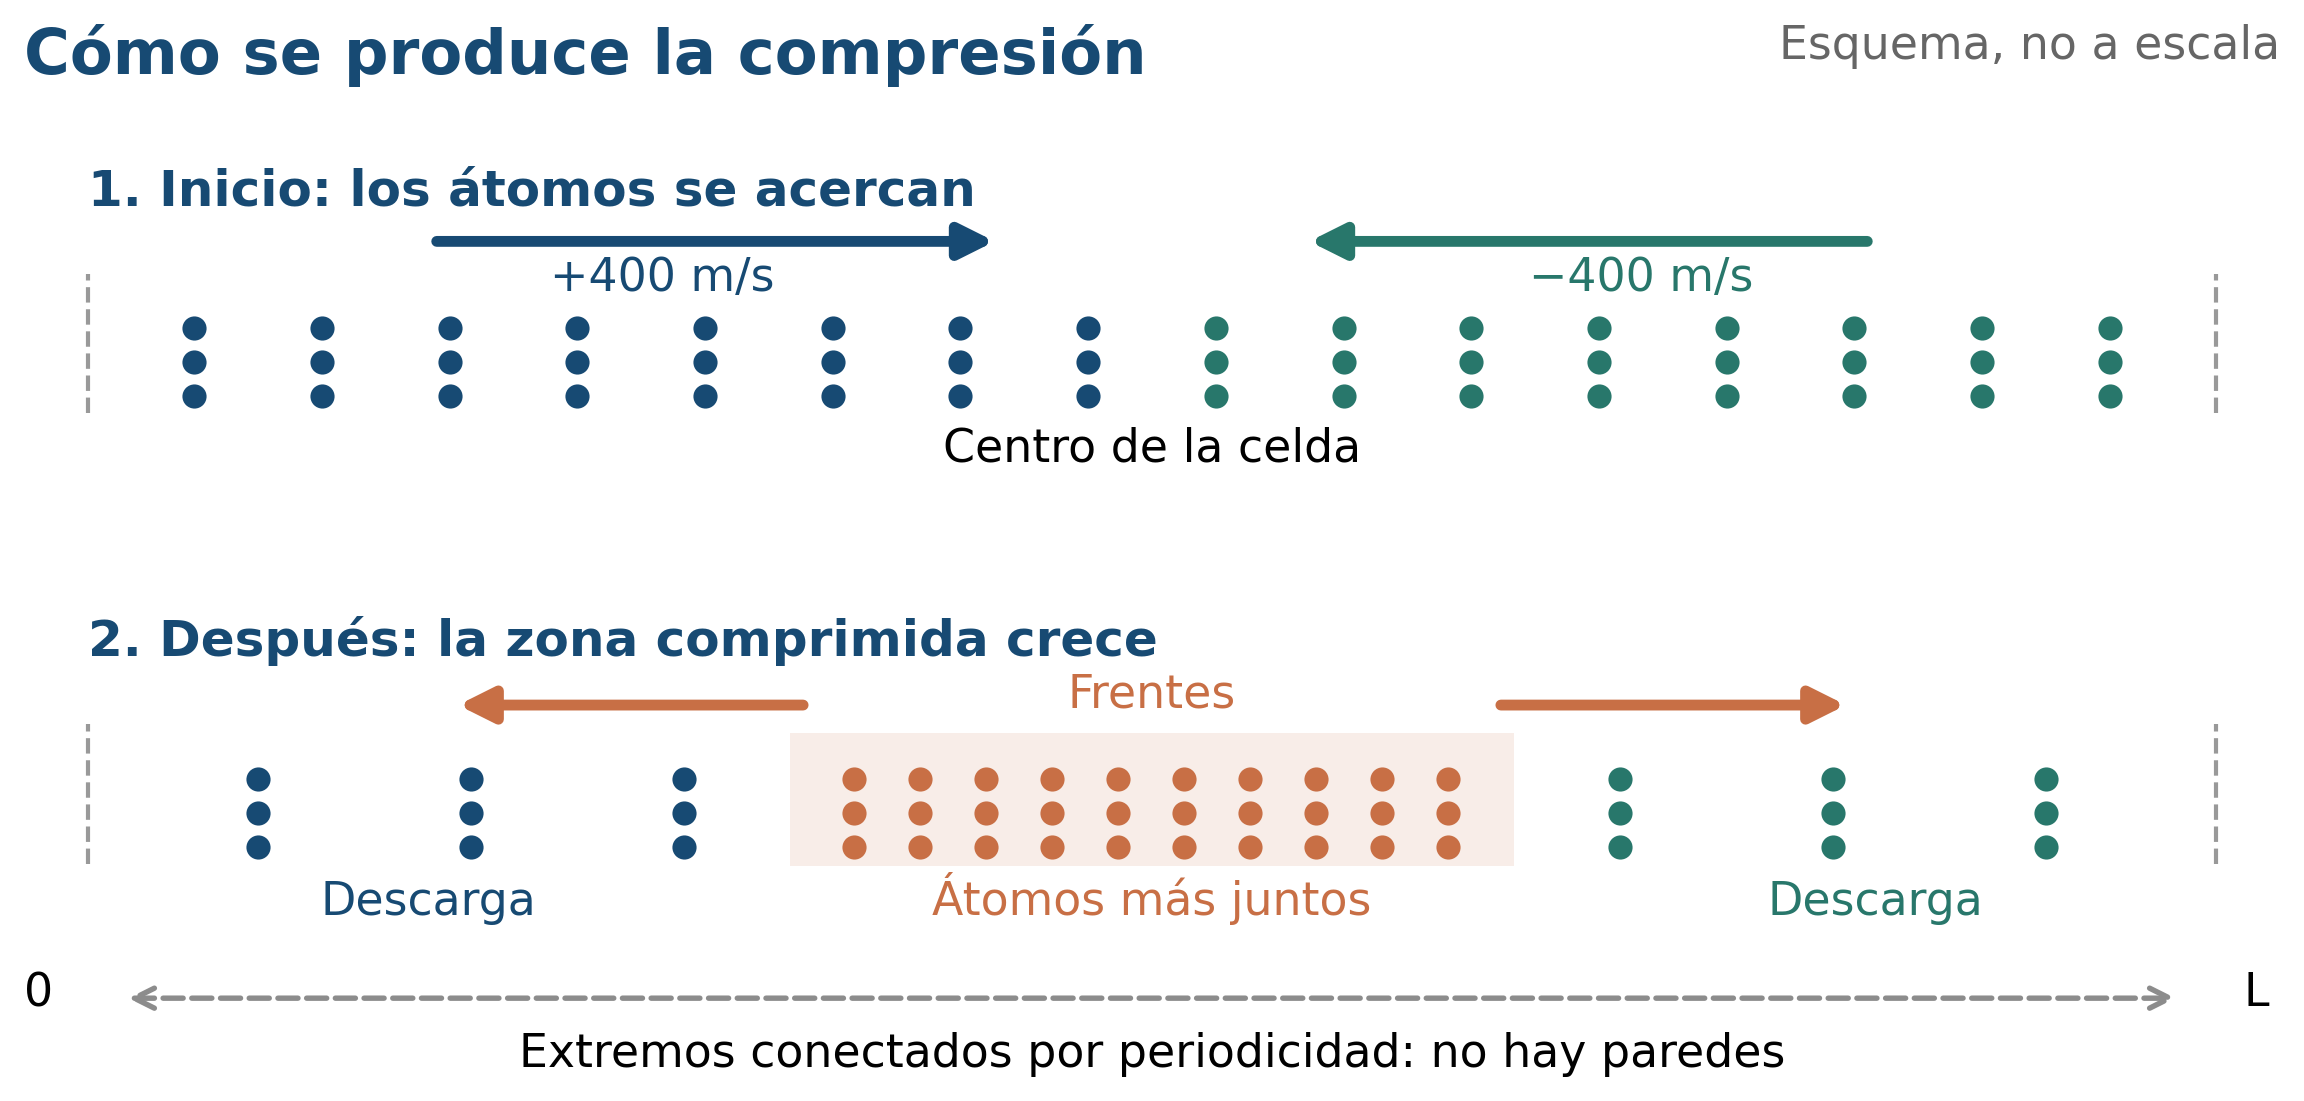
\includegraphics[width=0.90\linewidth]{esquema-choque.png}
\end{center}

\begin{minipage}[t]{0.47\linewidth}
\textbf{Al comenzar}\par
Cada mitad del cristal viaja hacia la otra a 400 m/s.
\end{minipage}\hfill
\begin{minipage}[t]{0.47\linewidth}
\textbf{Después del encuentro}\par
En el centro los átomos quedan más juntos y el flujo se frena.
\end{minipage}

\accion{}{Predice antes de ejecutar}
En el centro, la densidad \textbf{aumentará / disminuirá}.
¿Qué esperas de la velocidad media?
\respuesta

\accion{}{Actualiza el repositorio antes de buscar el ejemplo}
Abre una terminal en la raíz del repositorio que clonaste y ejecuta:
\begin{lstlisting}[style=terminal]
git pull --ff-only
\end{lstlisting}
Así descargas los cambios del código y los ejemplos. El programa instalado se
actualiza al recompilar y reinstalar, como se indica en la página 2.

\begin{pista}{Prepara tu carpeta de trabajo con el administrador de archivos}
Después de actualizar, copia \archivo{lpmd/examples/shock-wave} a un lugar de tu
preferencia. Dentro de tu copia, crea tres carpetas: \archivo{prueba},
\archivo{choque} y \archivo{tiempos}. Conserva los scripts junto a ellas.\par
Mi carpeta de trabajo: \rule{0.68\linewidth}{0.35pt}\par
Abre las terminales con \textit{Abrir en terminal} en la carpeta indicada en cada
paso. Así cada estudiante puede usar sus propias rutas.
\end{pista}

\newpage
\titulo{02 / COMPROBAR Y ACTUALIZAR LA INSTALACIÓN}{¿Tu instalación tiene OpenMP?}{Comprueba el programa instalado e incorpora los cambios descargados con Git.}

\accion{A}{Haz una prueba corta con tu instalación}
Copia \archivo{smoke.control} dentro de \archivo{prueba} y abre una terminal allí.
\begin{lstlisting}[style=terminal]
command -v lpmd
OMP_NUM_THREADS=2 OMP_DYNAMIC=FALSE OMP_DISPLAY_ENV=TRUE \
  lpmd smoke.control > run.log 2>&1
\end{lstlisting}
El primer comando muestra qué ejecutable usas. Anota su ruta:
\respuesta
El segundo pide dos hilos, evita que OpenMP ajuste ese número y guarda los mensajes
en \archivo{run.log}. Ábrelo con un editor de texto y busca:
\begin{tcolorbox}
\archivo{SIMULATION FINISHED}: la prueba terminó.\par
\archivo{OPENMP DISPLAY ENVIRONMENT} y \archivo{_OPENMP}: se cargó soporte OpenMP.\par
\archivo{OMP_NUM_THREADS = '2'}: se solicitaron dos hilos.
\end{tcolorbox}
\textbf{Si descargaste cambios del código o falta OpenMP, sigue el paso B.}
Si ya reinstalaste ese código y aparecen las tres señales, continúa en la página 3.
Si hubo un error de simulación, revísalo con el docente antes de continuar.

\accion{B}{Recompila e instala el código actualizado}
Busca la carpeta donde compilaste \textbf{este código de lpmd2}: puede llamarse
\archivo{build} u otro nombre. Debe contener \archivo{CMakeCache.txt}.
Ábrelo y comprueba que \archivo{CMAKE_INSTALL_PREFIX} corresponde a la instalación
anotada arriba; por ejemplo, \archivo{/usr/local} para \archivo{/usr/local/bin/lpmd}.
Estos comandos usan \archivo{Unix Makefiles}; comprueba el campo
\archivo{CMAKE_GENERATOR} del mismo caché. Si usaste otro generador,
consulta el README antes de continuar.

Abre una terminal \textbf{en esa carpeta de compilación} y ejecuta, una línea a la vez:
\begin{lstlisting}[style=terminal]
cmake . -DLPMD_ENABLE_OPENMP=ON -DCMAKE_BUILD_TYPE=Release
cmake --build . --target preinstall --parallel 4
sudo cmake --install .
\end{lstlisting}
El punto significa \textit{esta carpeta}; se conservan las rutas registradas por
CMake. La primera línea activa OpenMP. La segunda compila y prepara la instalación,
incluidas las copias \archivo{CMakeRelink.dir} cuando hacen falta; espera a que termine sin errores.
La tercera reinstala los archivos preparados.
\textbf{Compilar con \archivo{--parallel 4} y simular con cuatro hilos son decisiones distintas.}

\begin{pista}{Vuelve a comprobar}
Regresa a \archivo{prueba} y repite el paso A. Debe aparecer OpenMP y terminar la
corrida. Si la terminal encuentra otra copia de LPMD, usa la ruta completa del
recién instalado en lugar de \archivo{lpmd}. Si falta el caché o las rutas no
coinciden, revisa tu instalación con el docente.
\end{pista}

\newpage
\titulo{03 / EJECUTAR Y GRAFICAR}{Observar el choque}{Copia \archivo{shock.control} a la carpeta \archivo{choque} y abre una terminal allí.}

\begin{tcolorbox}
\begin{tabularx}{\linewidth}{@{}XXX@{}}
\textbf{6912 átomos de Ar} & \textbf{4000 pasos} & \textbf{2 ps físicos}\\
Cristal ordenado FCC & 0.5 fs por paso & $1\ \mathrm{ps}=1000\ \mathrm{fs}$
\end{tabularx}
\end{tcolorbox}

\begin{lstlisting}[style=terminal]
OMP_NUM_THREADS=4 OMP_DYNAMIC=FALSE \
  lpmd shock.control > run.log 2>&1
\end{lstlisting}
Usa 1, 2 o 4 hilos según los núcleos disponibles para tu trabajo. Espera a que vuelva
el indicador de la terminal y confirma \archivo{SIMULATION FINISHED} en el registro.
Se crean \archivo{shock.xyz}, \archivo{shock-monitor.dat} y \archivo{shock-final.dump}.

\accion{}{Transforma la trayectoria en dos gráficos}
En la misma terminal, ejecuta estas dos líneas. Python se usa aquí para
agrupar los átomos por posición y dibujar tus resultados:
\begin{lstlisting}[style=terminal]
python3 ../profiles.py shock.xyz --output perfiles.csv
python3 ../plot_results.py perfiles.csv
\end{lstlisting}
Abre \archivo{shock-profiles.png} con doble clic. Necesitas Python 3 y Matplotlib;
si falta este último, sigue la instalación indicada en el README.

\begin{center}
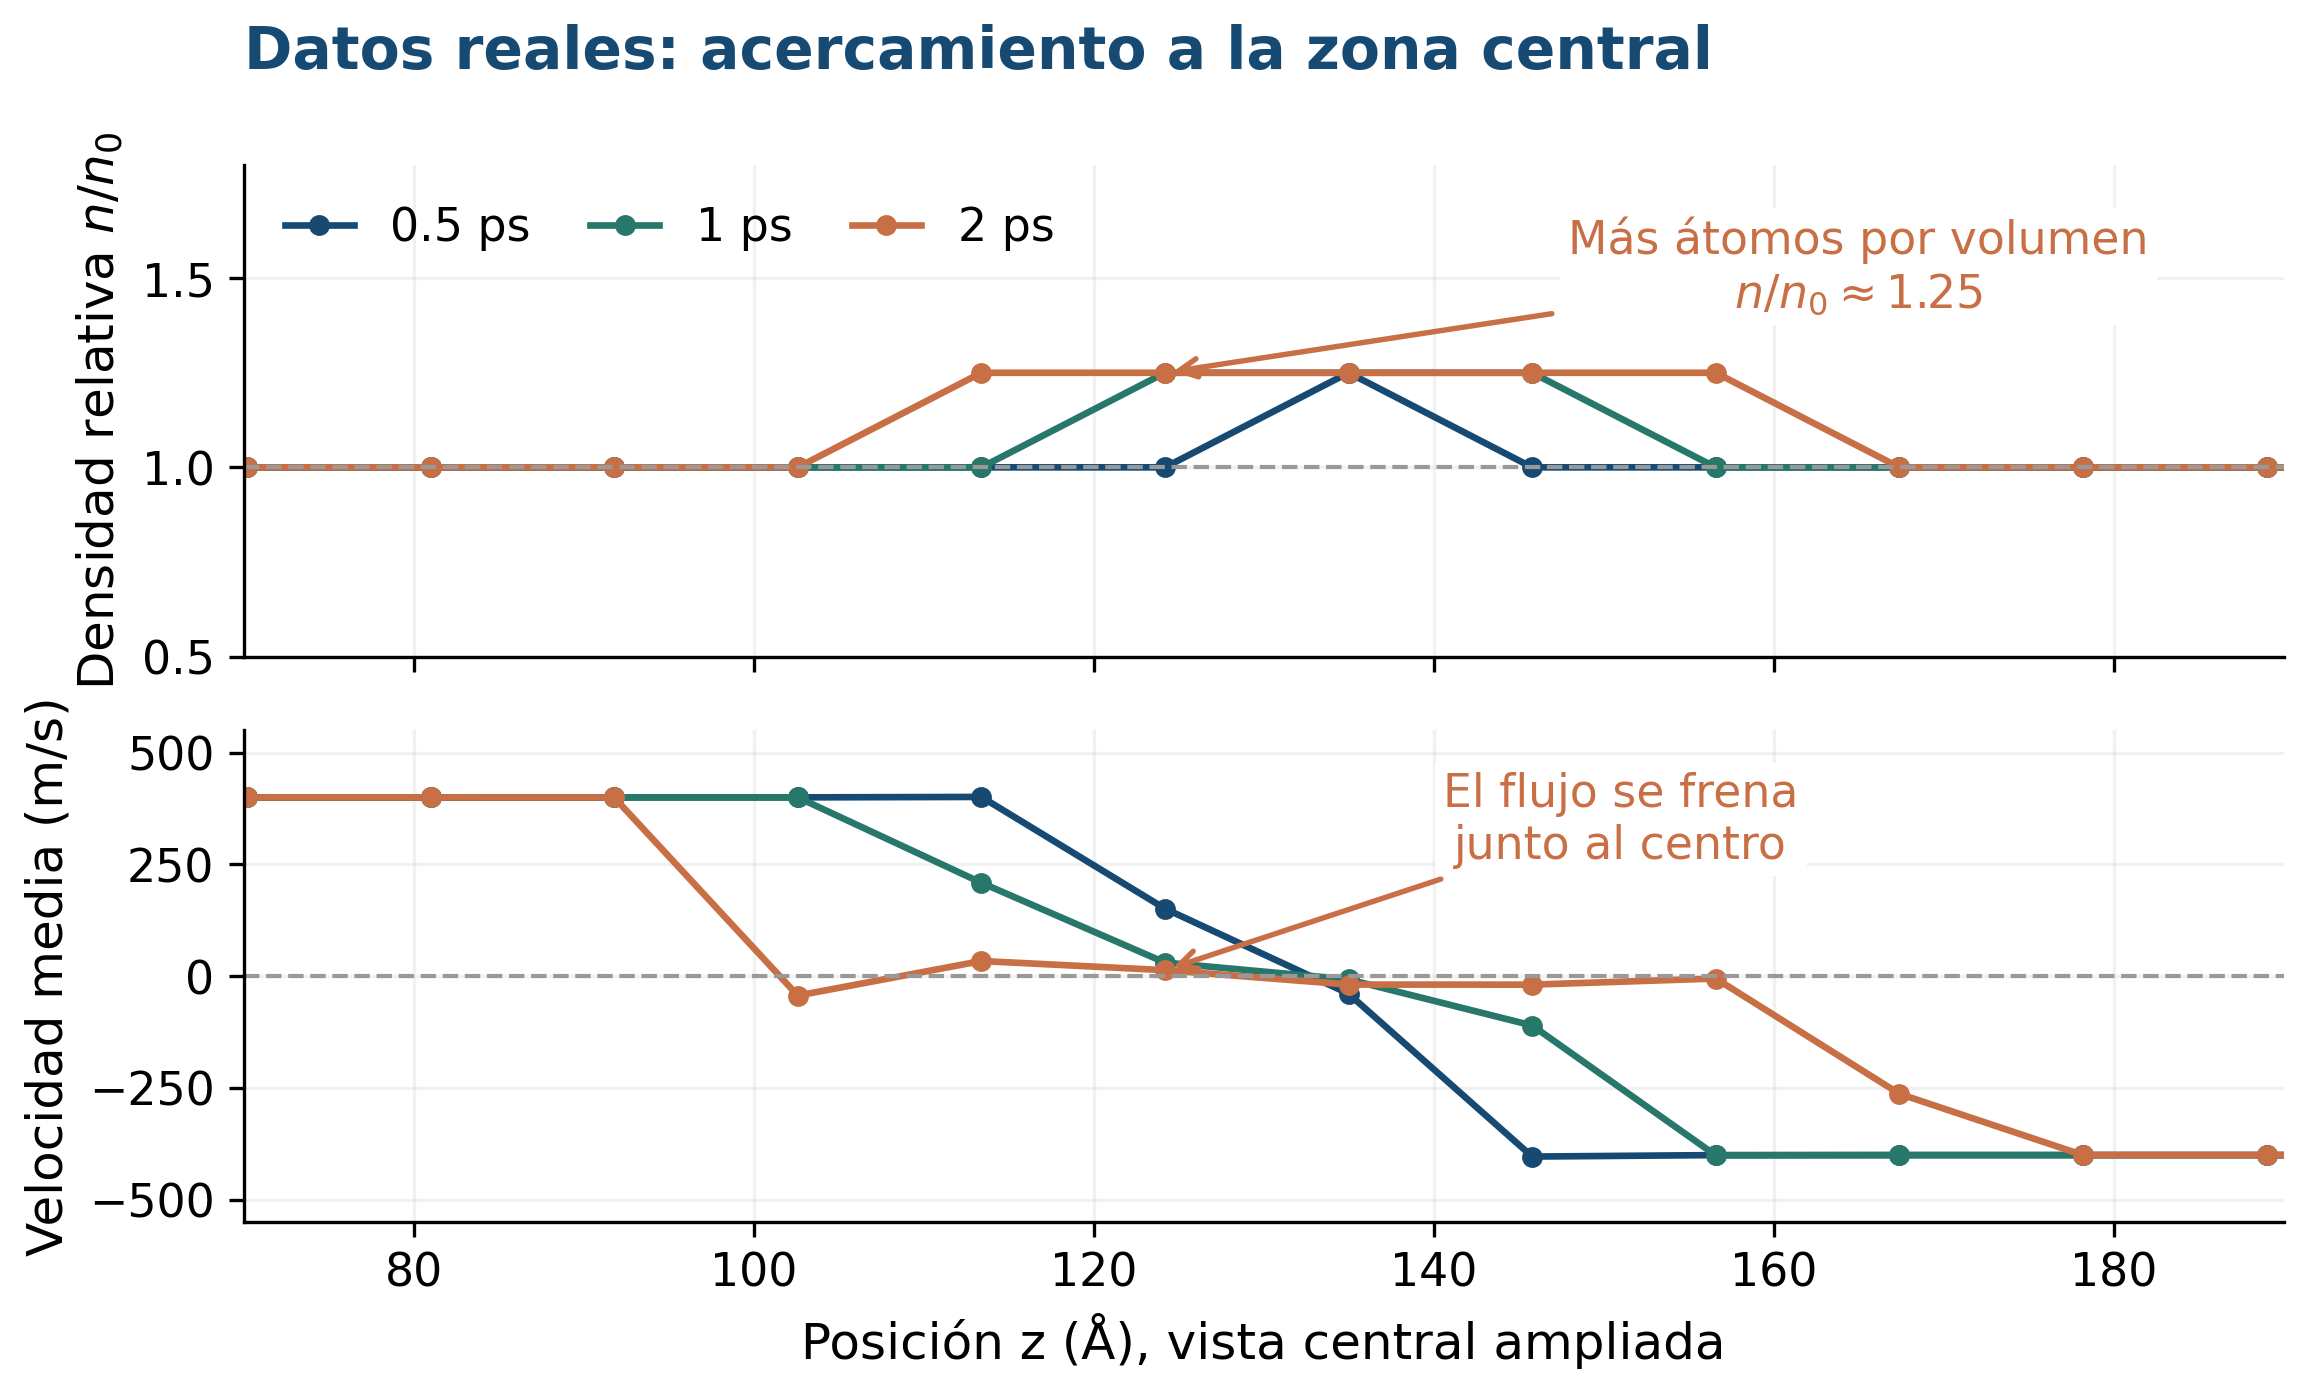
\includegraphics[width=0.84\linewidth]{perfiles.png}
\end{center}
{\small\color{gris}Referencia calculada con este ejemplo, ampliada alrededor del
centro. Tu figura muestra toda la celda. $n/n_0>1$ indica compresión; una velocidad
media cercana a cero indica que el flujo se frenó. Busca cómo crece esa zona.}

\newpage
\titulo{04 / MEDIR EL TIEMPO DE ESPERA}{Comparar 1, 2 y 4 hilos}{Mantén el mismo sistema. Cambia únicamente el número de hilos solicitados.}

\begin{center}
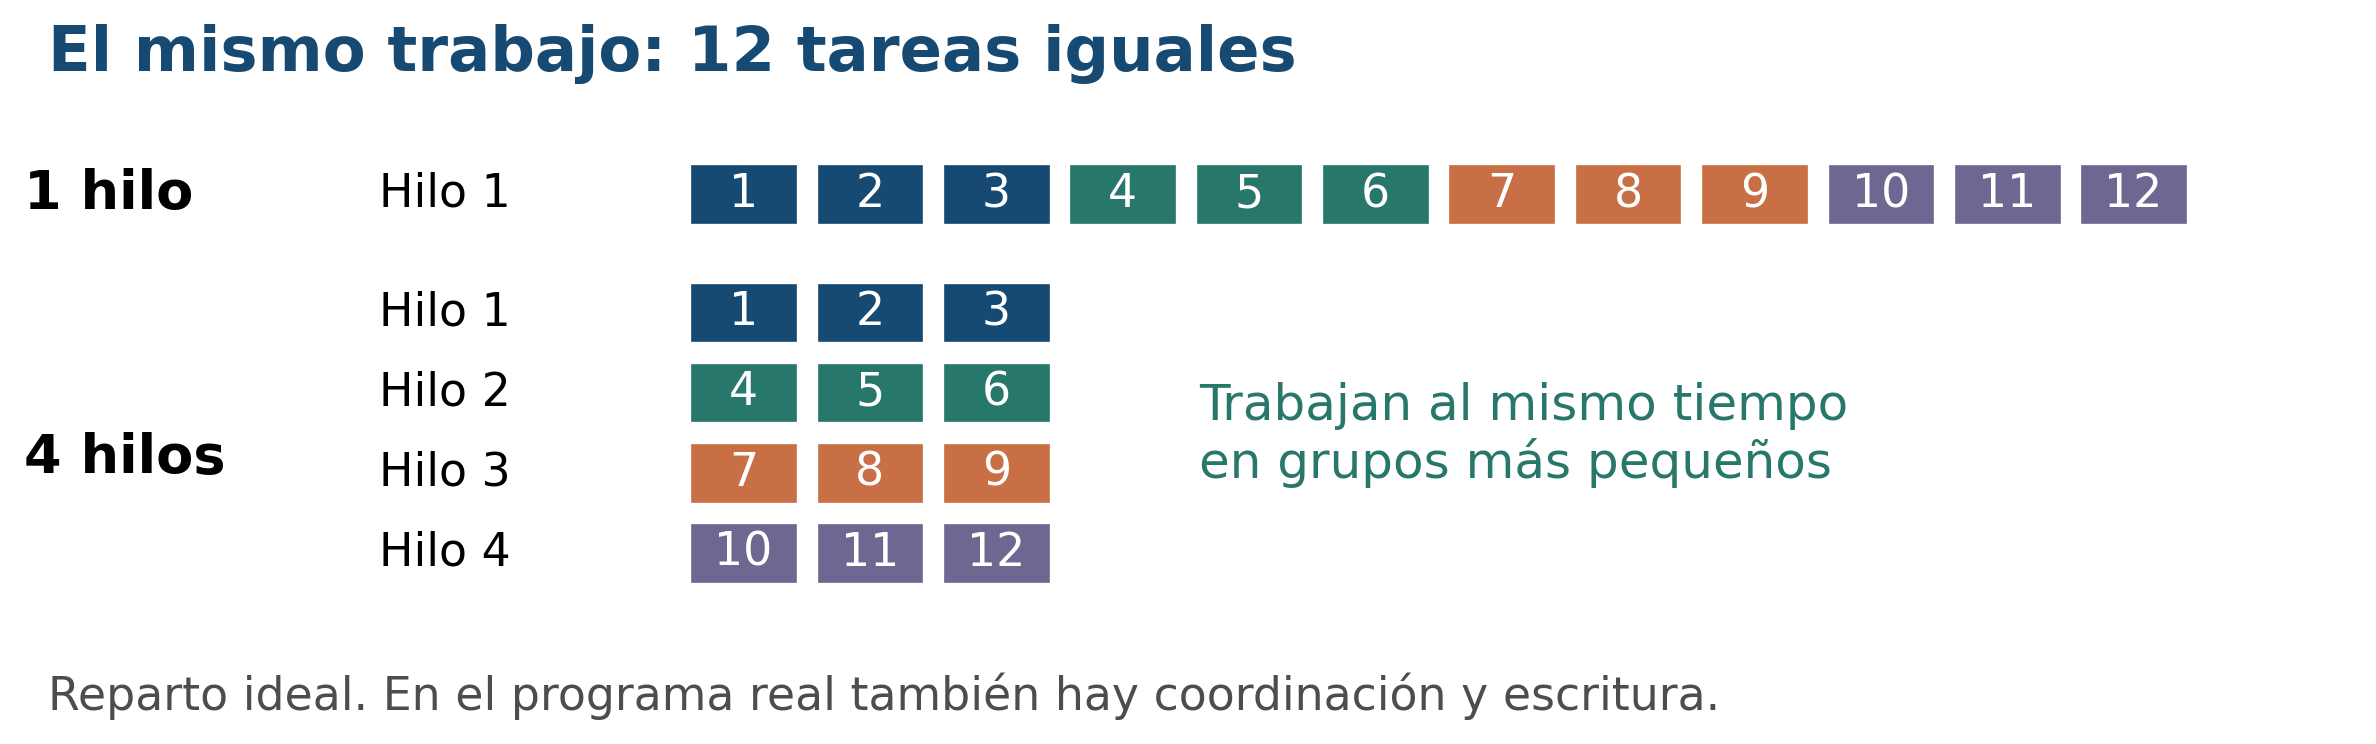
\includegraphics[width=0.87\linewidth]{hilos.png}
\end{center}

\accion{A}{Prepara una comparación breve}
Dentro de \archivo{tiempos}, crea \archivo{1-hilo}, \archivo{2-hilos} y
\archivo{4-hilos}. Copia \archivo{tiempos.control} en cada una.
Este control conserva los 6912 átomos y el paso de 0.5 fs; usa \textbf{200 pasos}
y omite XYZ en todos los casos. Así la medición dura menos y escribe menos datos.

\accion{B}{Ejecuta desde cada carpeta}
Abre una terminal en la carpeta correspondiente y usa su línea:
\begin{lstlisting}[style=terminal]
OMP_NUM_THREADS=1 OMP_DYNAMIC=FALSE lpmd tiempos.control > run.log 2>&1
OMP_NUM_THREADS=2 OMP_DYNAMIC=FALSE lpmd tiempos.control > run.log 2>&1
OMP_NUM_THREADS=4 OMP_DYNAMIC=FALSE lpmd tiempos.control > run.log 2>&1
\end{lstlisting}
\textbf{Haz tres corridas por número de hilos.} Tras cada una, abre \archivo{run.log},
confirma \archivo{SIMULATION FINISHED} y anota \archivo{Elapsed real time}.
Desde el administrador de archivos, renombra el registro como \archivo{r1.log},
\archivo{r2.log} o \archivo{r3.log} antes de repetir la línea. Las otras salidas de
esta comparación se reemplazan.

\begin{center}
\renewcommand{\arraystretch}{1.7}
\begin{tabular}{@{}ccccc@{}}
\toprule
Hilos & Corrida 1 (s) & Corrida 2 (s) & Corrida 3 (s) & Mediana (s)\\
\midrule
1 & \rule{1.9cm}{0.35pt} & \rule{1.9cm}{0.35pt} & \rule{1.9cm}{0.35pt} & \rule{1.9cm}{0.35pt}\\
2 & \rule{1.9cm}{0.35pt} & \rule{1.9cm}{0.35pt} & \rule{1.9cm}{0.35pt} & \rule{1.9cm}{0.35pt}\\
4 & \rule{1.9cm}{0.35pt} & \rule{1.9cm}{0.35pt} & \rule{1.9cm}{0.35pt} & \rule{1.9cm}{0.35pt}\\
\bottomrule
\end{tabular}
\end{center}

\begin{pista}{Compara con justicia}
La \textbf{mediana} es el valor del medio tras ordenar los tres tiempos.
Usa \textbf{real}, que mide espera; \textit{user} y \textit{system} suman tiempo de CPU.
Deja terminar una corrida antes de iniciar otra y evita otros cálculos simultáneos.
Si dispones de menos de cuatro núcleos, mide solo las filas que puedas usar.
\end{pista}

\newpage
\titulo{05 / INTERPRETAR}{¿Qué aprendemos de los resultados?}{Trabaja con tus perfiles y con las medianas que acabas de medir.}

\accion{1}{Relaciona densidad y movimiento}
En tu gráfico, a 2 ps y cerca del centro, leo aproximadamente:\par
$n/n_0=$ \rule{2cm}{0.4pt}\qquad
velocidad media $=$ \rule{2cm}{0.4pt} m/s.\par
¿Coincide con tu predicción? ¿Cómo cambia el ancho de la zona comprimida?
\respuesta

\accion{2}{Calcula cuánto se acelera el programa}
\[
S_p=\frac{\text{mediana con 1 hilo}}{\text{mediana con }p\text{ hilos}}.
\]
Con 2 hilos: $S_2=$ \rule{2cm}{0.4pt}\qquad
Con 4 hilos: $S_4=$ \rule{2cm}{0.4pt}\par
Si $S=2$, la simulación tarda la mitad. ¿La mejora es proporcional al número de hilos?
Da una posible razón para lo que observaste.
\respuesta

\begin{center}
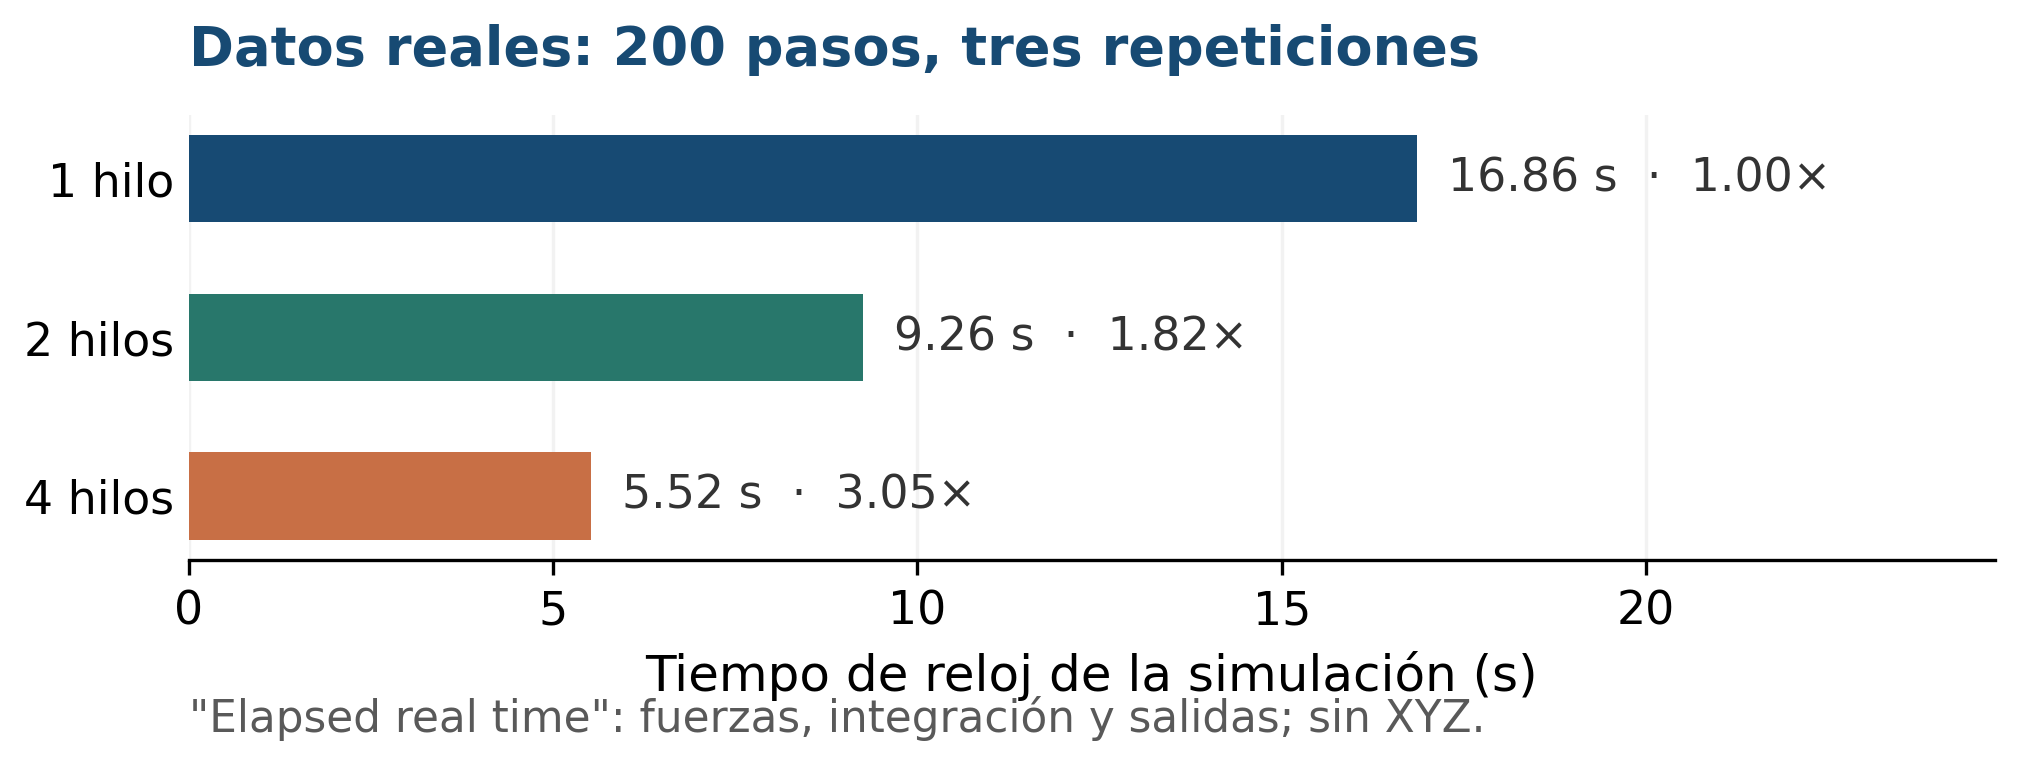
\includegraphics[width=0.85\linewidth]{tiempos.png}
\end{center}
{\small\color{gris}Referencia de un equipo: medianas de tres corridas de 200 pasos,
leyendo \archivo{Elapsed real time} como en la página 4. Tus tiempos pueden ser distintos.}

\accion{3}{Distingue los dos relojes}
El choque completo representa \textbf{2 ps físicos}. ¿Usar más hilos cambia esos
2 ps o cambia lo que esperas frente al computador?
\respuesta

\begin{pista}{Entrega breve}
Entrega tu gráfico de perfiles, la tabla de tiempos y estas tres respuestas.
Indica procesador, número de hilos y ruta del ejecutable usado. Conserva los
registros para poder revisar la comparación.
\end{pista}
{\small\color{gris}\textbf{Para interpretar:} el modelo frío y periódico produce
compresión central y descarga en los extremos. La temperatura global incluye el
movimiento colectivo; no mide por sí sola el calentamiento local.}

\end{document}
